\documentclass{beamer}

\usepackage{beamer_macros}
\addbibresource{../contact_metastability.bib}

\setbeamertemplate{section in toc}[sections numbered]
\setbeamertemplate{subsection in toc}[subsections numbered]


\mode<presentation>
{
  \useoutertheme{infolines}
  \useinnertheme{default}
  \usecolortheme{beaver}
}

\title{Metastability for the Contact Process on $\integer$, Part 1.}
\subtitle{Following \cite{schonmann_metastability_1985}}
\author{O.~Lynch\inst{1}}

\institute[Universiteit Utrecht]
{
  \inst{1}%
  Department of Mathematics \\
  Universiteit Utrecht
}

\date{\today}

\newtheorem*{proposition}{Proposition}

\newcommand{\ep}{\varepsilon}
\newcommand{\ignore}[1]{}
\newcommand{\rb}{\ignore{[}]}

\begin{document}

\begin{frame}
  \titlepage
\end{frame}

\begin{frame}{Outline}
  \tableofcontents
\end{frame}

\section{Introduction}

\begin{frame}{Introduction}
  \tableofcontents[currentsection]
\end{frame}

\subsection{Metastability}

\begin{frame}{Informal Metastability}
  \begin{itemize}
    \item Markov process $\xi_{N}(t) \ins \integer$, ``infected states at time $t$''
    \pause
    \item As $N$ goes to $\infty$, looks like figure~\ref{fig:coarse_grain}.
  \end{itemize}
  \begin{figure}
    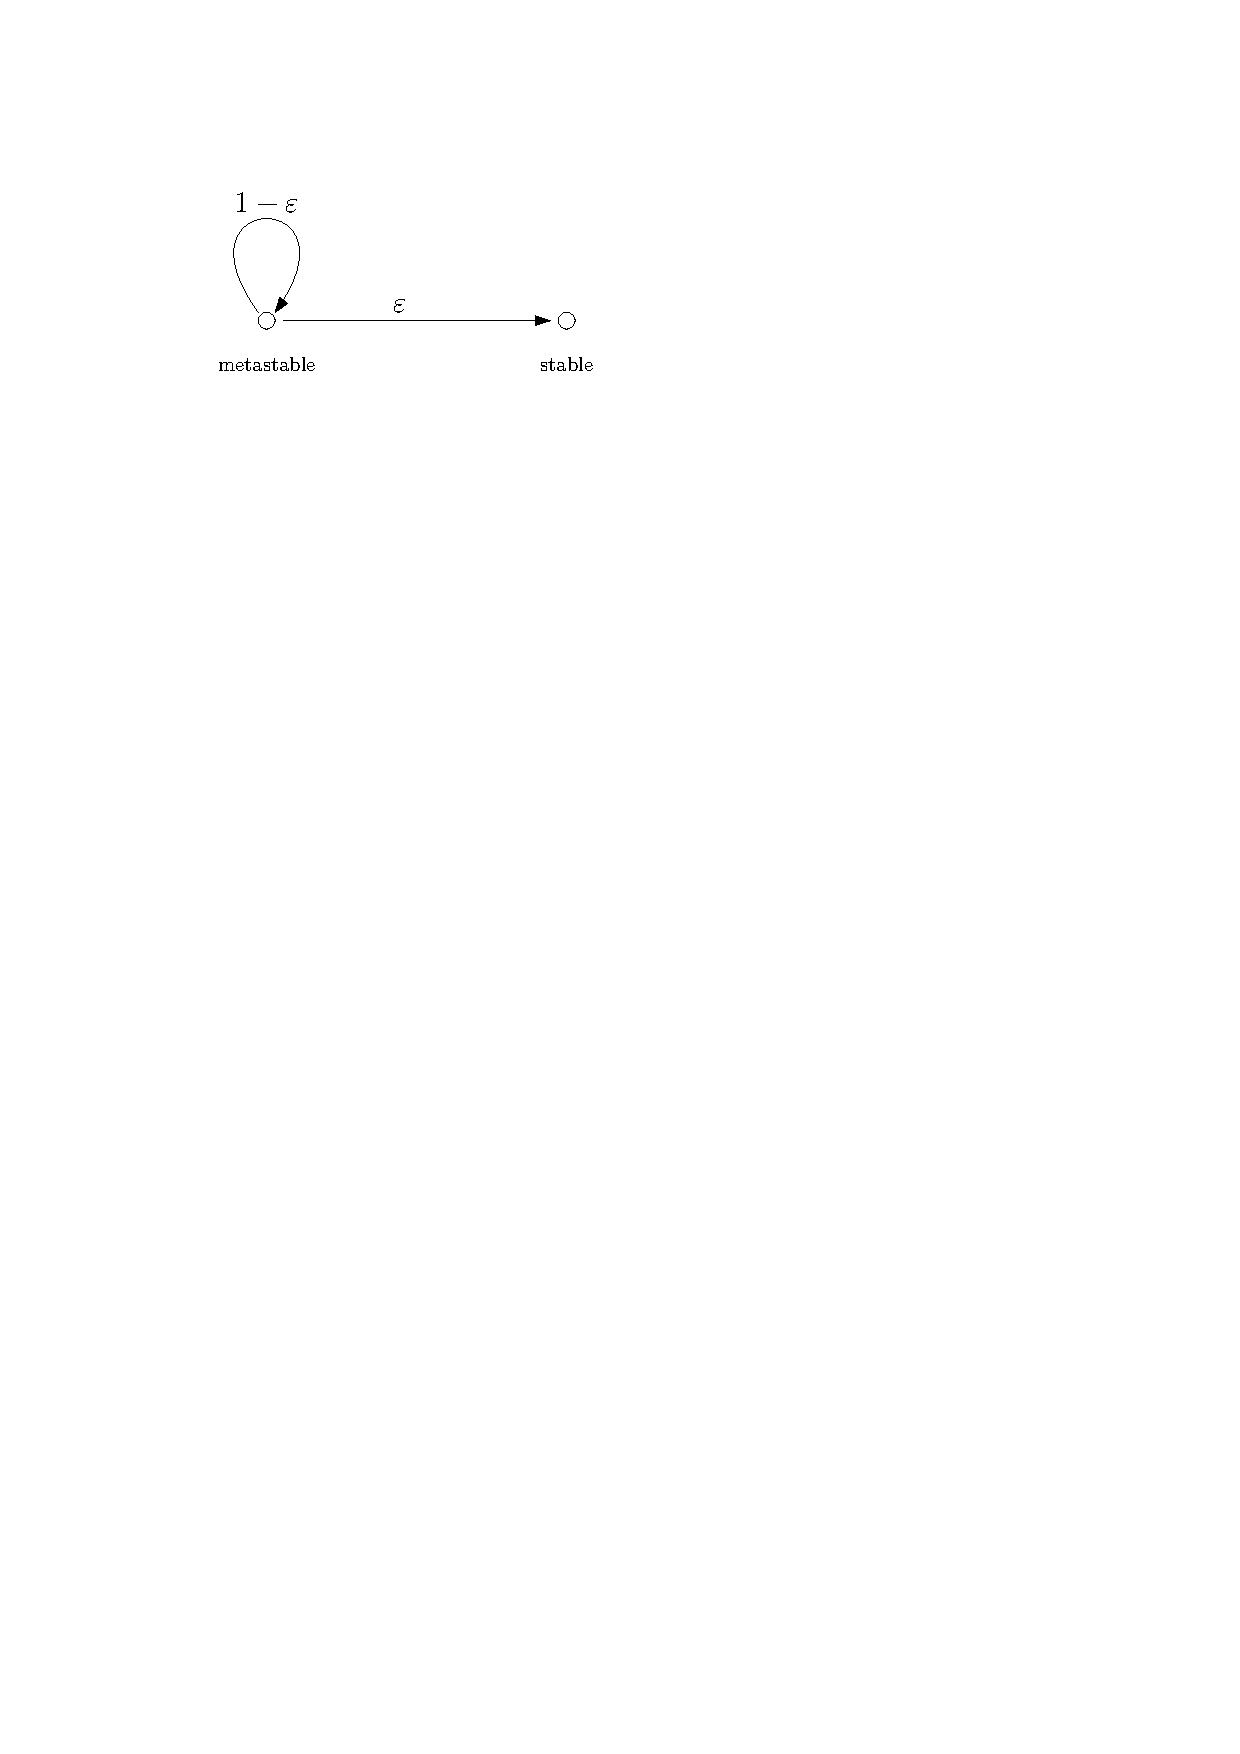
\includegraphics[width=0.7\pagewidth]{metastable_coarse_grain.pdf}
    \caption{Coarse Graining as $N \to \infty$}
    \label{fig:coarse_grain}
  \end{figure}
\end{frame}

\begin{frame}{Formal Metastability}
  \begin{enumerate}
    \item Exponential hitting time
    \begin{itemize}
      \item There is a ``trap state'', with hitting time $T_{N}$
      \item Asymptotically as $N \to \infty$, $T_{N}$ has an exponential distribution.
    \end{itemize}
    \pause
    \item Quasi-stationary distribution before hitting time
    \begin{itemize}
      \item There is a ``approximate invariant distribution'' $\mu$
      \item Up until $T_{N}$, temporal means of $X_{N}(t)$ approximate $\mu$
    \end{itemize}
  \end{enumerate}
\end{frame}

\subsection{Contact Process}

\begin{frame}{Contact Process, Generator Definition}
  \begin{itemize}
    \item $\xi(t)$ is a Markov process taking values in $2^{\integer} = \powerset(\integer)$
    \item Characterized by
      \begin{equation}
        \label{eq:definition_contact_proc}
        Lf(\eta) = \sum_{x} c(x,\eta)(f(\eta^{x}) - f(\eta))
      \end{equation}
    \item With rates
      \begin{equation}
        \label{eq:contact_proc_rates}
        c(x,\eta) = \begin{cases}
          1 & \qif* \eta(x) = 1 \\
          \lambda(\eta(x-1) + \eta(x+1)) & \qotherwise*
        \end{cases}
      \end{equation}
  \end{itemize}
\end{frame}

\begin{frame}{Contact Process, Percolation Structure Definition}
  \begin{itemize}
    \item (show animation 1)
    \pause
    \item 3 processes for each site $x \in \integer$: $P_{x}$ (rate 1), $P_{x \to x+1}$ and $P_{x \to x-1}$ (both rate $\lambda$).
    \pause
    \item $\xi^{A}(t)$ is the set of $x \in \integer$ such that there is a path $(y,0) \to (x,t)$ for $y \in A$.
    \pause
    \item A path is... \pause easier to see intuitively in than write down formally
    \pause
    \item Percolation structure is very useful for proofs
  \end{itemize}
\end{frame}

\begin{frame}{Smaller Processes}
  \begin{itemize}
    \item $\xi_{B}^{A}(t)$ is the set of $x \in B$ such that there is a path $(y,0) \to (x,t)$ with $y \in A$ and the path not leaving $B$
          \pause
    \item Superscript: ``starts in'', subscript: ``contained in''
          \pause
    \item If $B$ is omitted, assumed to be $\integer$. If $A$ is omitted, assumed to be $B$.
          \pause
    \item Special cases
    \begin{itemize}
      \item $\xi_{N}(t) = \xi_{[-N,N]}(t)$
      \item $\xi_{[-N,\infty)}(t)$
      \item $\xi_{(-\infty,N\rb}(t)$
    \end{itemize}
          \pause
    \item We are interested in metastability for $\xi_{N}(t)$, with trap state $\emptyset$.
  \end{itemize}
\end{frame}

\section{Crash Course in Contact Process}

\begin{frame}{Crash Course in Contact Process}
  \tableofcontents[currentsection]
\end{frame}

\subsection{Toolbox}

\begin{frame}{Critical $\lambda$}
  \begin{itemize}
    \item Survival/extinction of $\xi(t)$ depends on infection rate $\lambda$
          \pause
    \item For $\lambda < \lambda_{c}$, goes extinct in finite time a.s. (unique ergodic measure $\delta_{\emptyset}$)
          \pause
    \item For $\lambda > \lambda_{c}$, two extremal invariant measures: $\delta_{\emptyset}$ and $\mu$
          \pause
    \item This also holds for $\xi_{[-N,\infty)}(t)$ and $\xi_{(-\infty,N]}(t)$
  \end{itemize}
\end{frame}

\begin{frame}{Monotone Convergence}
  \begin{itemize}
    \item $\Prob(\xi^{A}(t) \cap B \neq \emptyset)$ is a nonincreasing function of $t$.
      \pause
    \item Converges to $\mu_{A}(\set{\eta \st \eta \cap B \neq \emptyset})$, where $\mu_{B}$ is the invariant measure of $\xi$ started in state $B$.
  \end{itemize}
\end{frame}

\begin{frame}{Self-duality}
  As long as $A$ or $B$ is finite, then for all $t$.
  \begin{equation}
    \Prob(\xi^{A}(t) \cap B \neq \emptyset) = \Prob(\xi^{B}(t) \cap A \neq \emptyset)
  \end{equation}
  \pause
  ``The probability of reaching somewhere in $B$ starting from $A$ is the same as the probability of reaching somewhere in $A$ starting from $B$''
  \pause
  Specifically, for $A$ finite
  \begin{equation}
    \Prob(\xi^{A}(t) \neq \emptyset) = \Prob(\xi(t) \cap A \neq \emptyset)
  \end{equation}
\end{frame}

\begin{frame}{Consequence of Monotone Convergence + Self-duality}
  \begin{align*}
    \Prob(\xi^{A}(t) \neq \emptyset, \forall t > 0) &= \limas_{s \to \infty} \Prob(\xi^{A}(t) \neq \emptyset, \forall s \geq t > 0) \\
                                 &= \limas_{s \to \infty} \Prob(\xi^{A}(s) \neq \emptyset) \\
                                 &= \limas_{s \to \infty} \Prob(\xi(s) \cap A \neq \emptyset) \\
                                 &= \mu(\set{\eta \st \eta \cap A \neq \emptyset})
  \end{align*}
\end{frame}

\begin{frame}{Characterizing $\mu$}
  \begin{itemize}
    \item $\mu$ is translation invariant
          \pause
    \item For $\lambda > \lambda_{c}$, given $\ep$, we can find $n(\ep)$ such that $\mu(\eta | \eta \cap [1,n(\ep)] \neq \emptyset) > 1 - \ep$
          \pause
    \item Therefore, we can find $n(\ep)$ so that if you start out in $[1,n(\ep)]$, you are almost sure to survive.
          \pause
    \item It turns out that you can generalize this: if you start out \emph{with at least $n(\ep)$} elements, you are almost sure to survive.
  \end{itemize}
\end{frame}

\subsection{Review}

\begin{frame}
  What have we learned so far?
  \begin{itemize}
    \item An intuition for metastability --- two key properties
          \pause
    \item How to use the percolation structure to construct many related contact processes
          \pause
    \item Some miscellaneous useful facts about the contact process
          \pause
          \begin{itemize}
            \item Critical $\lambda$
                  \pause
            \item Monotone convergence
                  \pause
            \item Self-duality
                  \pause
            \item How an infection can persist forever with high probability: it has to start out with enough sites infected
          \end{itemize}
  \end{itemize}
\end{frame}

\section{Theorem 1}

\begin{frame}{Theorem 1}
  \tableofcontents[currentsection]
\end{frame}

\subsection{Overview}

\begin{frame}{Goals}
  \begin{theorem}
    Let \[ T_{N} = \inf\set{t \st \xi_{N}(t) = \emptyset} \]
    Then for $\lambda > \lambda_{c}$
    \[ \frac{T_{N}}{\E T_{N}} \to[w] \expDist(1) \]
    That is, it converges to $\expDist(1)$ \emph{in distribution}.
  \end{theorem}
  \pause
  \begin{itemize}
    \item Not feasible to give whole proof
          \pause
    \item Instead, will give strategy and then give detailed proof of just one part
  \end{itemize}
\end{frame}

\begin{frame}{Strategy Part 1}
  \begin{itemize}
    \item Use $\beta_{N}$ instead of $\E T_{N}$, where $\beta_{N}$ is unique number such that
    \[ \Prob(T_{N} > \beta_{N}) = \e^{-1} \]
          \pause
    \item Let $G_{N}(t) = \Prob\left[ \frac{T_{N}}{\beta_{N}} > t\right]$ be the tail distribution for $T_{N} / \beta_{N}$
          \pause
    \item(note that $\set{ \frac{T_N}{\beta_N} > t} = \set{\xi_{N}(\beta_{N}t) \neq \emptyset}$)
          \pause
    \item Prove that
          \[ \limas_{N \to \infty} \abs{G_{N}(t)G_{N}(s) - G_{N}(t+s)} = 0 \]
    \item The only function with $f(t+s) = f(t)f(s)$ and $\int_{0}^{\infty} f(t) \dd{t} = 1$ is $f(t) = e^{-t}$.
  \end{itemize}
\end{frame}

\begin{frame}{Strategy Part 2}
  \begin{itemize}
    \item Use a set $F_{b} \ins \powerset([-N,N])$ of ``sufficiently dense'' initial conditions
    \pause
    \item If we are not in $F_{b}$, then we are most likely already extinct. Therefore, the probability that we end up in $F_{b}$ at time $\beta_{N}t$ is approximately $G_{N}(t)$
    \pause
    \item Starting from $A \in F_{b}$ is ``just as good'' as starting from $[-N,N]$, so if we end up in $A \in F_{b}$ at time $\beta_{N}t$, then we have approximately $G_{N}(s)$ chance of still being alive at time $\beta_{N}(s+t)$.
    \pause
    \item Put together, these two imply that $G_{N}(t)G_{N}(s) \sim G_{N}(t+s)$
  \end{itemize}
\end{frame}

\subsection{An Excerpt from Schonman Op. 1}

\begin{frame}{Into the Unknown}
  \begin{itemize}
    \item Show that $\Prob[T_{N} = T_{N}^{A}] > 1 - \ep$ when $A \in F_{b}$, for sufficiently large $N$ and $b$. (i.e., $A \in F_{b}$ is ``just as good'' as $[-N,N]$)
    \item Let
          \[F_{b} = \set{A \in \integer \st \frac{\abs{A \cap [-b,-1]}}{b} \geq \frac{\rho}{2}, \frac{\abs{A \cap [1,b]}}{b} \geq \frac{\rho}{2}}\]
    \item ``sufficiently dense on both sides''
    \item $\rho = \Prob[\xi^{\set{0}}(t) \neq \emptyset, \forall t] = \mu(\eta \st \eta(0) = 1)$.
  \end{itemize}
\end{frame}

\begin{frame}
  \begin{itemize}
    \item Let $n = n(\ep)$ large enough so that starting out with $n$ infected sites will let the epidemic persist forever with probability $1 - \ep/2$
          \pause
    \item Then if $b \rho/2 > n(\ep)$, for $A$ in $F_{b}$ starting in $[1,b] \cap A$ or $[-b,-1] \cap A$ will persist forever with probability $1 - \ep/2$
          \pause
    \item Let $E$ be the event that $\xi_{[-N,\infty)}^{A\cap[-b,-1]}(t)$ and $\xi_{(-\infty,N]}^{A \cap [1,b]}(t)$ persist forever (the invariant distribution for $[-N,\infty)$ is the same as that for $\integer$)
          \pause
    \item $\Prob(E) > 1 - \ep$
          \pause
    \item Therefore, we are done if in $E$, $T_{N} = T_{N}^{A}$.
  \end{itemize}
\end{frame}

\begin{frame}
  \begin{itemize}
    \item Define two stopping times
    \begin{align*}
      U &= \inf\set{t \st N \in \xi_{[-N,\infty)}^{A \cap [-b,-1]}(t)} \\
      V &= \inf\set{t \st -N \in \xi_{(-\infty,N\rb}^{A \cap [1,b]}(t)}
    \end{align*}
  \end{itemize}
  \pause
  \begin{figure}
    \centering
   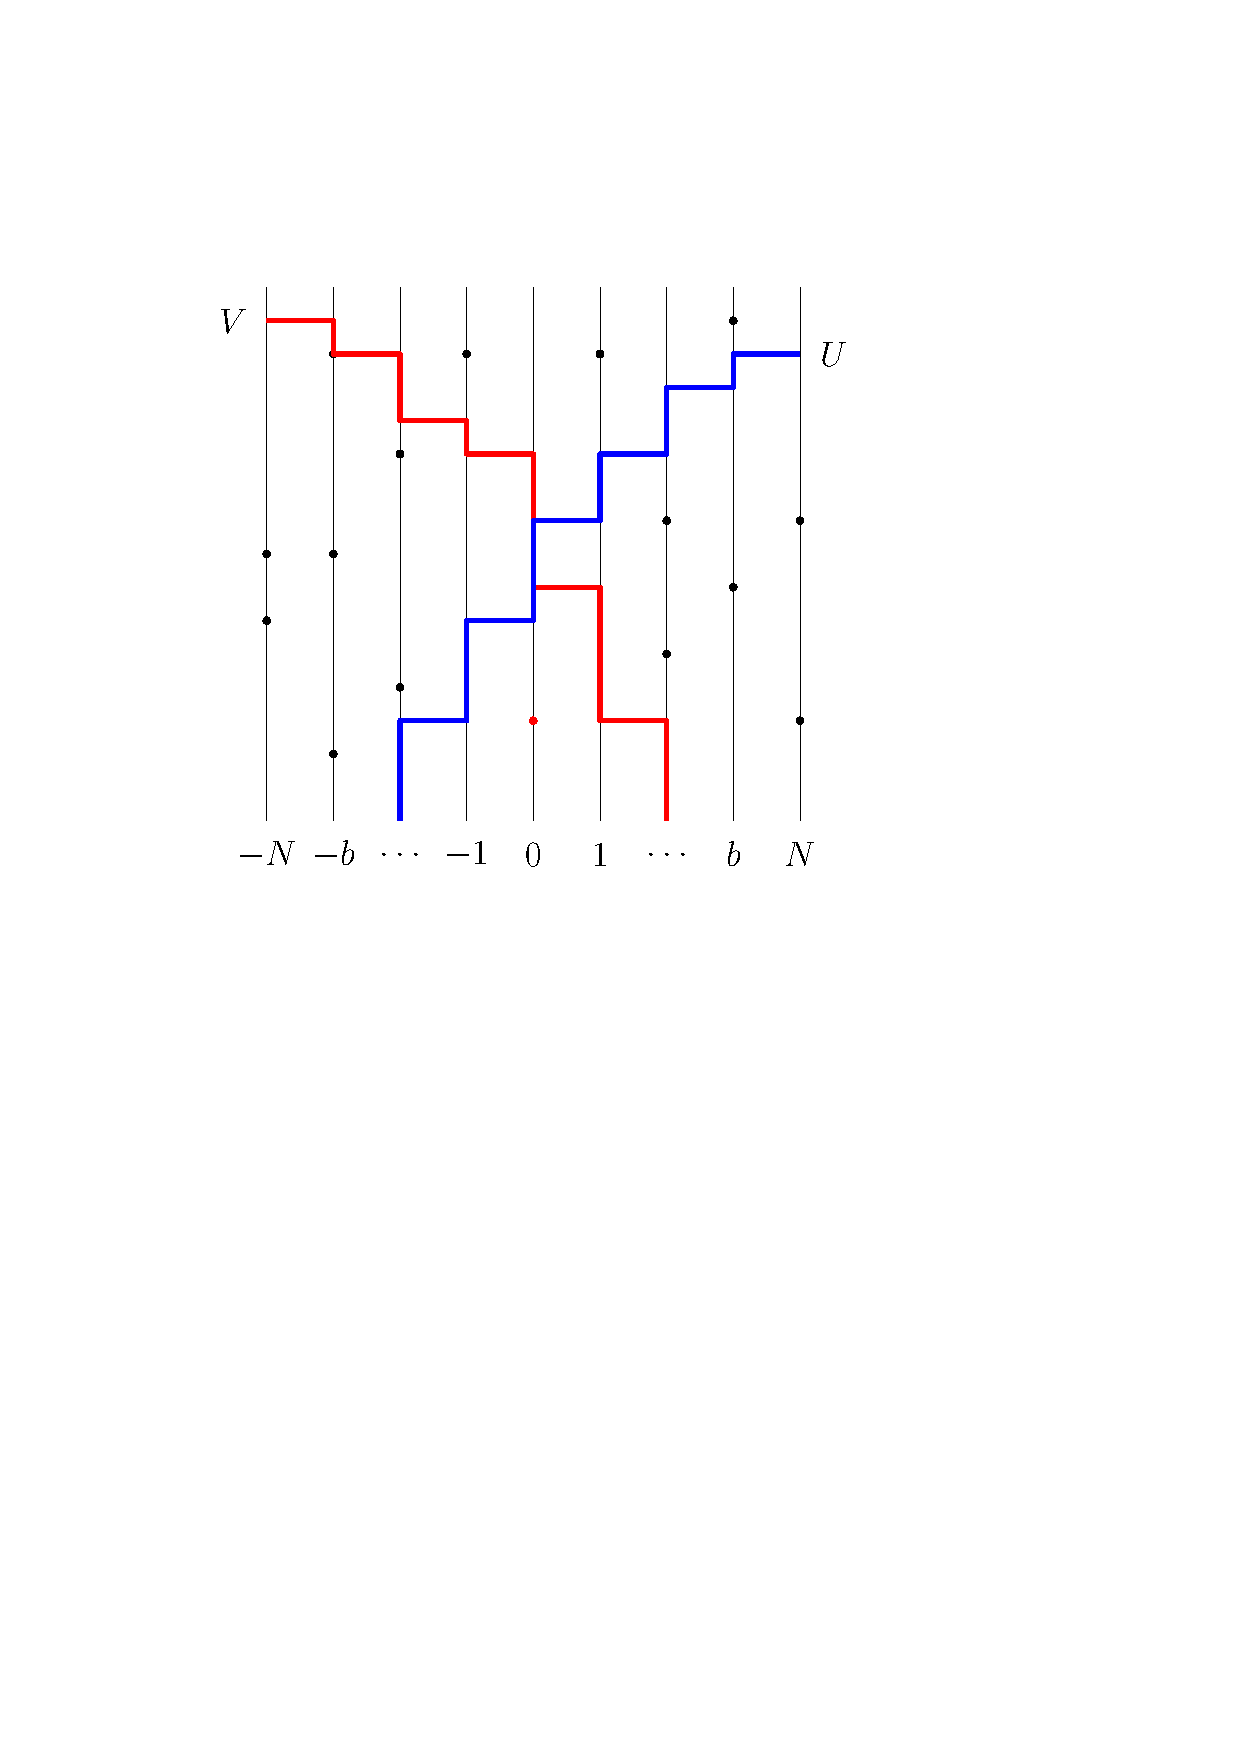
\includegraphics[width=0.5\textwidth]{U_V.pdf}
 \end{figure}
\end{frame}

\begin{frame}
  \begin{itemize}
    \item $U$ and $V$ are almost surely finite on $E$.
    \item At time $U$, $\xi_{N}^{A}$ is alive, because $\xi_{N}^{A}(U) \supset \xi_{[-N,\infty)}^{A \cap [-b,-1]}(t)$, and similarly for $V$, so $T_{N} \geq T_{N}^{A} > \max(U,V)$
  \end{itemize}
\end{frame}

\begin{frame}
  \begin{itemize}
    \item After $U$ and $V$, there is a path from $[-b,-1] \cap A$ to $N$, and a path from $[1,b] \cap A$ to $-N$. Intuitively, one of those paths intersects any path from $x \in [-N,N]$ to $y \in \xi_{N}(t)$.
  \end{itemize}
  \begin{figure}
    \centering
    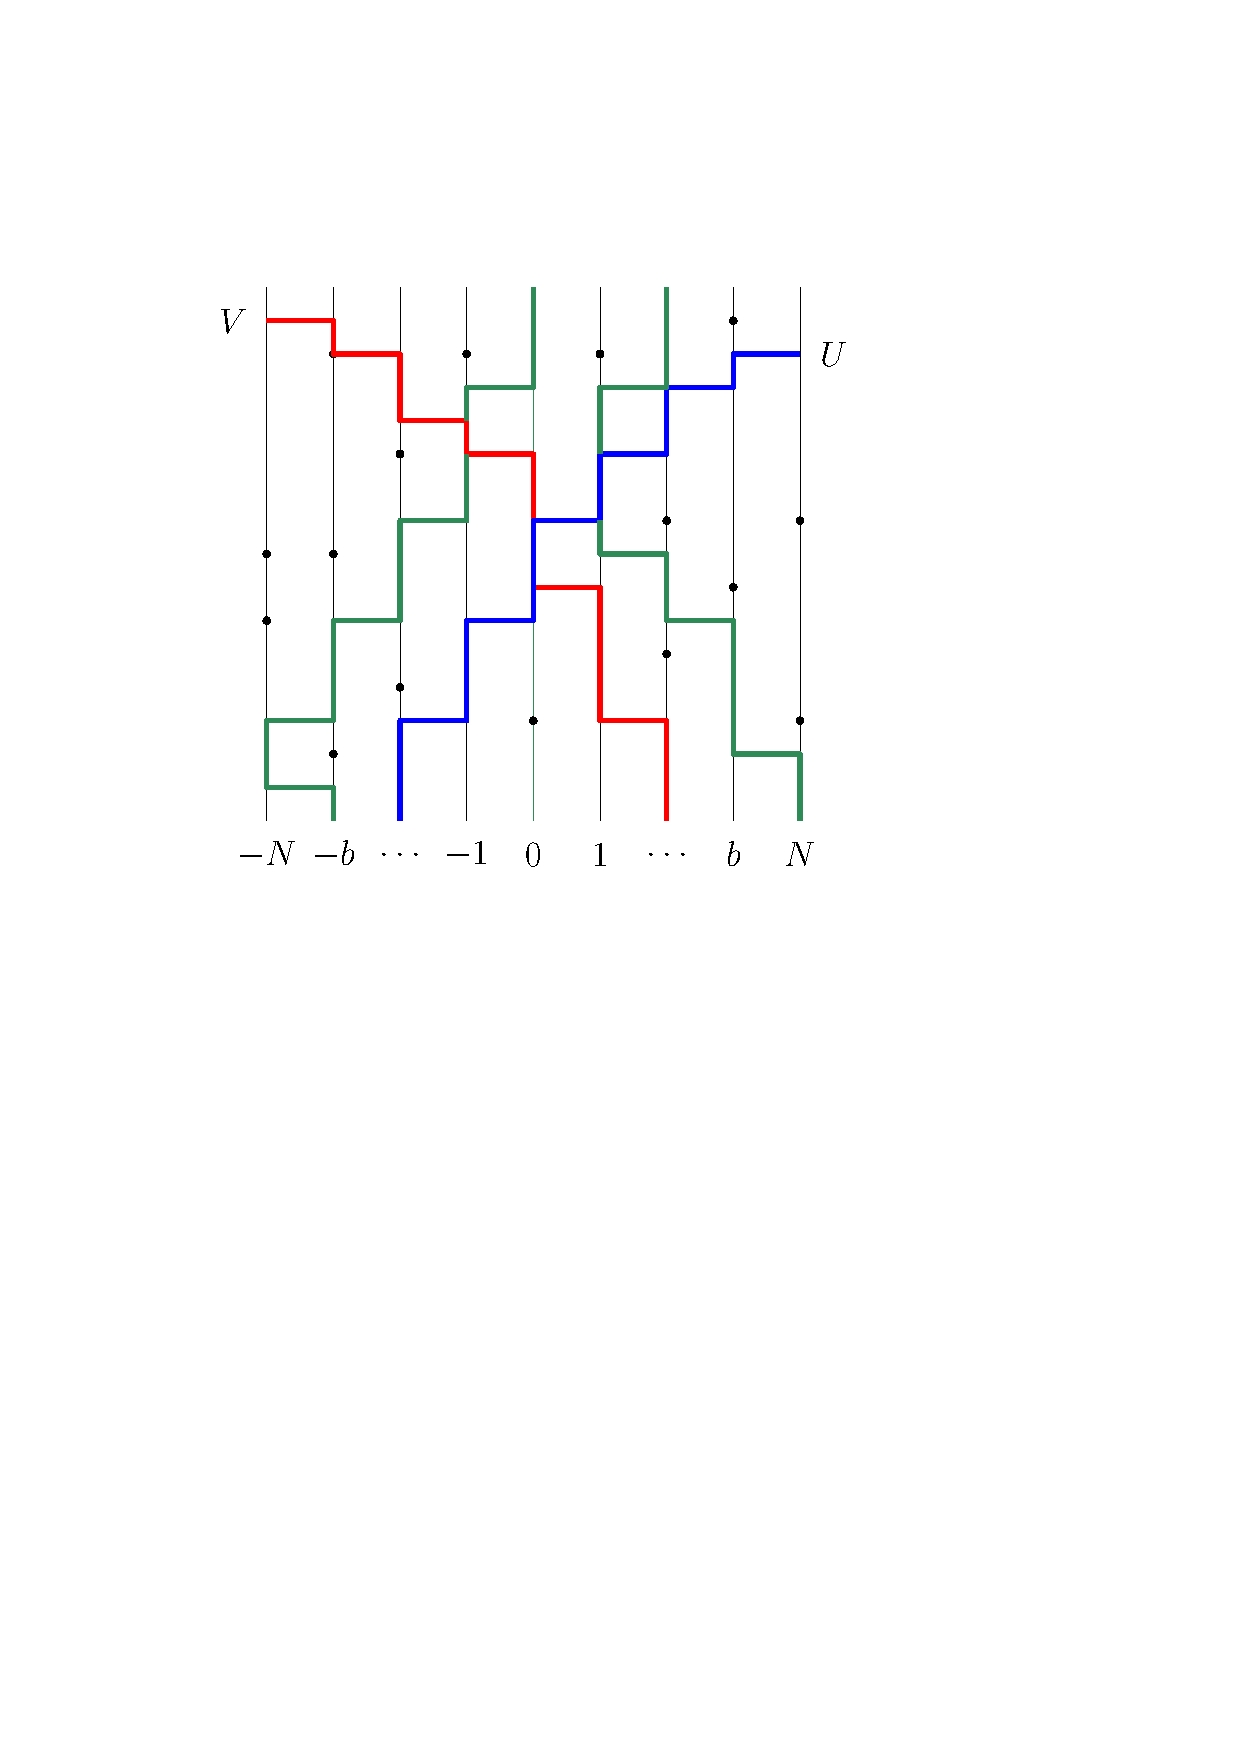
\includegraphics[width=0.5\textwidth]{U_V_blocked.pdf}
  \end{figure}
\end{frame}

\begin{frame}
  \begin{itemize}
    \item For $t > \max(U,V)$, $\xi_{N}(t) = \xi_{N}^{A}(t)$
    \item Therefore, $T_{N} = T_{N}^{A}$ on $E$, and we have shown that $\Prob(T_{N} = T_{N}^{A}) > 1 - \ep$.
  \end{itemize}
\end{frame}

\subsection{Conclusion}

\begin{frame}{Summary}
  We have learned
  \begin{itemize}
          \pause
    \item What metastability is
          \pause
    \item Basic properties of the contact process
          \pause
    \item A rough sketch of how the contact process is metastable (part 1)
          \pause
    \item What working with the contact process in practice looks like
  \end{itemize}
\end{frame}

\begin{frame}{Citations}
  \printbibliography
\end{frame}

\end{document}
